\chapter{Development Methodology}

\section{Introduction}

The development methodology defines the software engineering principles, lifecycle framework, and tooling used to build the Sentio platform. Because Sentio combines real-time WebSockets, visual slide authoring, and generative artificial intelligence, an iterative \textbf{Agile Scrum} methodology was chosen to support continuous prototyping, testing, and improvement.

\section{Agile Scrum Framework}

Rather than trying to build the entire system in one massive, sequential phase, the Agile approach breaks the project into short, manageable development cycles called sprints. This iterative process allowed us to build working features quickly, test them immediately, and refine the architecture as technical challenges arose.

The project was organized into six two-week sprints. Each sprint followed a clear cycle of backlog prioritization, sprint planning, feature implementation, and automated testing.

\begin{figure}[H]
    \centering
    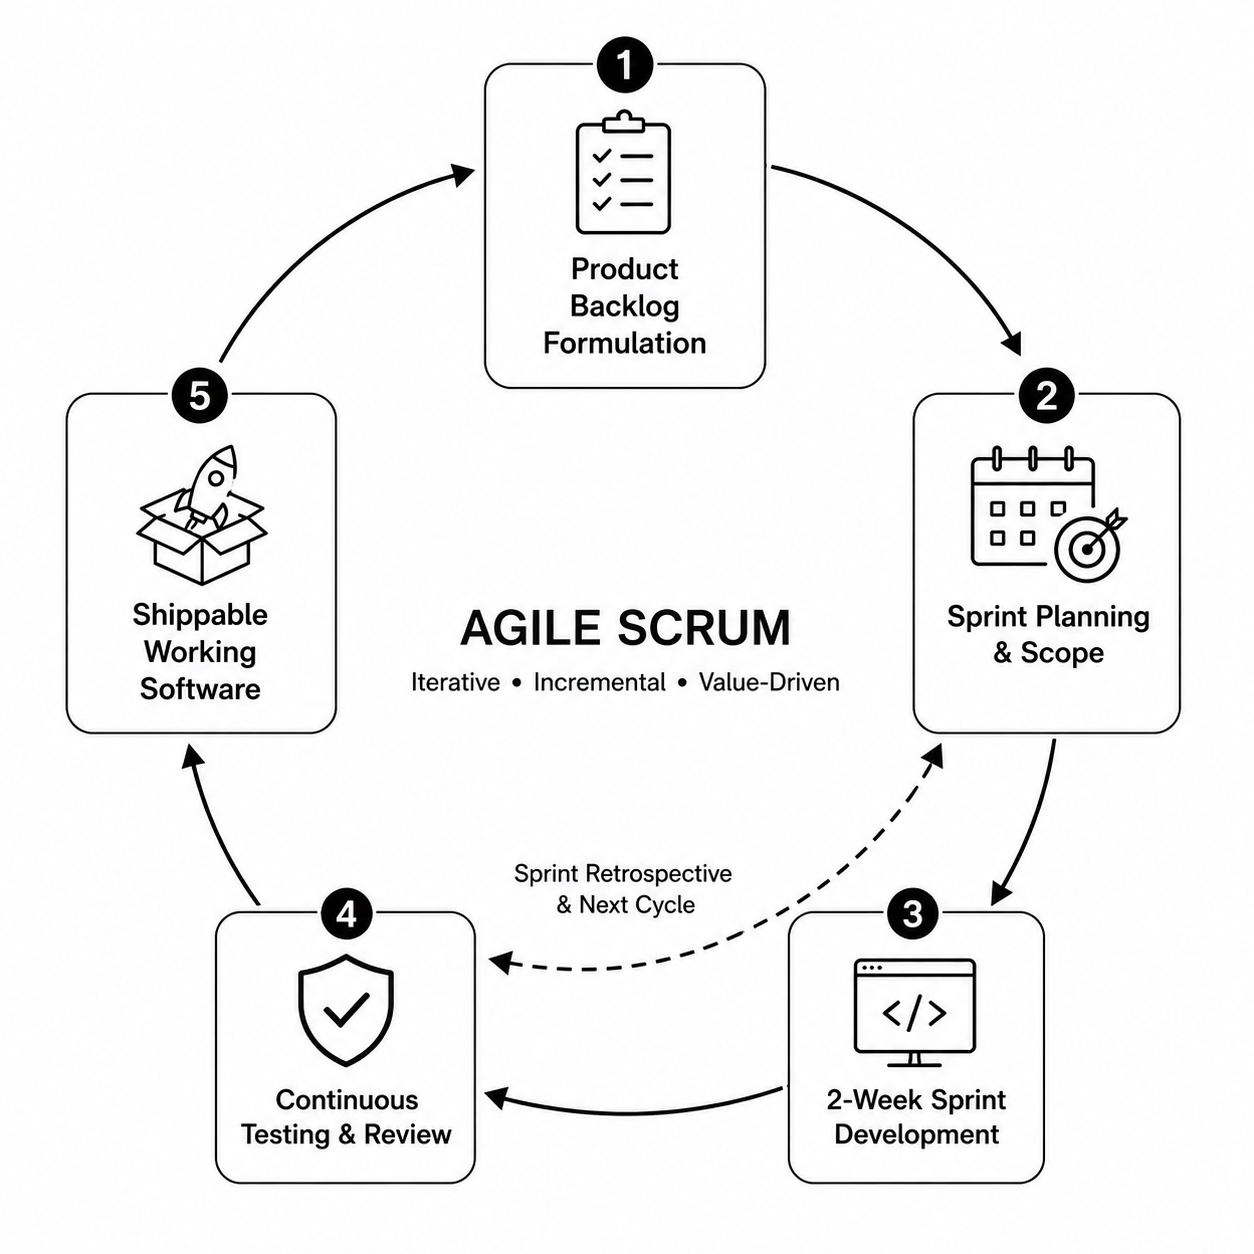
\includegraphics[width=0.85\textwidth]{figures/AgileCycle.png}
    \caption{Agile Scrum Development Cycle for Sentio}
    \label{fig:scrumcycle}
\end{figure}

\subsection{Sprint Milestones}

The core functionality of Sentio was built across distinct sprint milestones:

\begin{itemize}
    \item \textbf{Sprint 1 (Core Foundation):} Setting up the monorepo workspace, defining shared TypeScript contracts, implementing user registration, secure JWT login, and connecting to MongoDB.
    \item \textbf{Sprint 2 (Presentation Studio):} Building the user dashboard, slide management system, and the 16:9 visual canvas editor with automatic debounced saving.
    \item \textbf{Sprint 3 (Real-Time Engine):} Implementing the Socket.IO server, room-based broadcasting, presenter live controls, and the participant mobile joining screen.
    \item \textbf{Sprint 4 (Interactive Elements):} Developing the full suite of interactive components—quizzes with timers, live polls, word clouds, star ratings, and the competitive leaderboard.
    \item \textbf{Sprint 5 (AI Integration \& Reports):} Integrating Groq AI with the LLaMA 3.3 model for instant slide generation and adding downloadable PDF session reports.
    \item \textbf{Sprint 6 (Testing \& Hardening):} Writing unit tests with Jest, testing API security, checking mobile responsiveness, and finalizing documentation.
\end{itemize}

\section{Monorepo Architecture}

Sentio is organized as a monorepo using npm workspaces. This architecture keeps the frontend, backend, and shared data models cleanly organized in one repository while ensuring full type safety across the entire application:

\begin{verbatim}
Sentio/
├── apps/
│   ├── frontend/         # Next.js 15 App (React 19 + Tailwind CSS)
│   └── backend/          # Node.js + Express + Socket.IO API
├── packages/
│   └── shared/           # Shared TypeScript interfaces & socket events
└── docs/                 # Project documentation
\end{verbatim}

The \texttt{shared} package acts as a single source of truth. Both the frontend and backend import data structures and socket event names directly from this package, preventing mismatch bugs during development.

\section{Technology Stack Justification}

Table~\ref{tab:techstack} provides an overview of the core technologies chosen for Sentio and the practical reasons for their selection.

\begin{table}[H]
\centering
\caption{Technology Stack Summary}
\label{tab:techstack}
\begin{adjustbox}{max width=\textwidth}
\begin{tabular}{lll}
\toprule
\textbf{Layer} & \textbf{Technology} & \textbf{Reason for Selection} \\
\midrule
Frontend & Next.js 15 \& React 19 & Fast performance, modern App Router, and clean UI components \\
Styling & Tailwind CSS & Utility-based CSS for rapid, responsive interface styling \\
Backend & Node.js \& Express.js & Asynchronous, event-driven runtime ideal for web APIs \\
Real-Time & Socket.IO v4 & Fast bidirectional communication for live audience responses \\
Database & MongoDB \& Mongoose & Flexible document storage well-suited for slide data \\
AI Engine & Groq (LLaMA 3.3) & High-speed AI inference for fast slide and quiz creation \\
PDF Reports & PDFKit & Server-side PDF creation for downloadable session summaries \\
Security & JWT \& Bcrypt & Standard secure user authentication and password hashing \\
\bottomrule
\end{tabular}
\end{adjustbox}
\end{table}
